
\section{L'équipe Rhoban et la compétition de football robotique RoboCup}

Les travaux développés dans cette thèse ont tout du long été
fortement guidés et inspirés par la participation 
de l'équipe de robotique \textit{Rhoban} à la compétition 
internationale de la \textit{RoboCup}.
Cette compétition a grandement orienté la construction et le
développement de l'équipe, en motivant depuis 2011 ses progrès constants.\\

La RoboCup est une compétition annuelle internationale
de robotique ayant vu le jour en 1997.
À la suite de la victoire la même année de l'ordinateur \textit{Deep Blue} conçu
par IBM sur le champion d'échec Garry Kasparov, 
les fondateurs de la RoboCup ont proposé le défi technologique 
suivant (\cite{kitano_robocup_1998}) : 
\begin{quote}
\textit{
Qu'une équipe de robots humanoïdes entièrement autonomes batte, en respectant 
les règles standards de la FIFA, la meilleure équipe de football mondiale
d'ici le milieu du 21\up{e} siècle.
}
\end{quote}
Depuis la déclaration de cet objectif très ambitieux, 
plusieurs ligues de football robotique ont été créées. 
Chacune explorant et progressant sur un aspect différent 
du problème\footnote{D'autre ligues poursuivant d'autres 
ambitions existent également.}.

\begin{figure}[htb]
    \centerfloat
    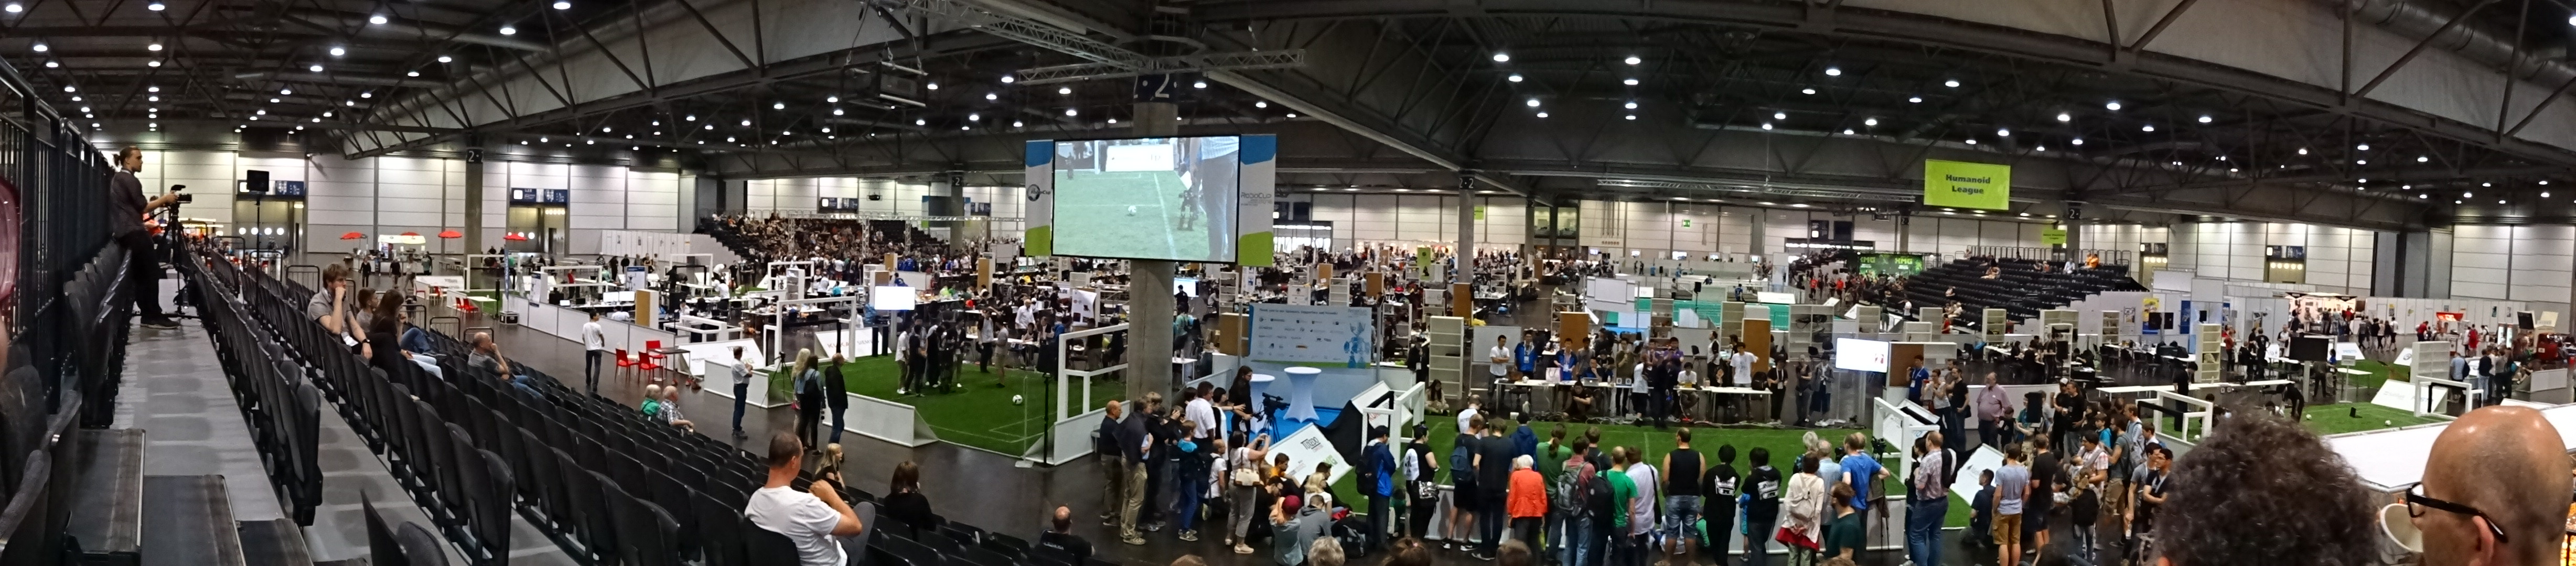
\includegraphics[trim={40cm 0cm 0cm 0cm},clip,width=1.30\linewidth]{../media/robocup_view.jpg}
    \begin{subfigure}{0.43\paperwidth}
        \centering
        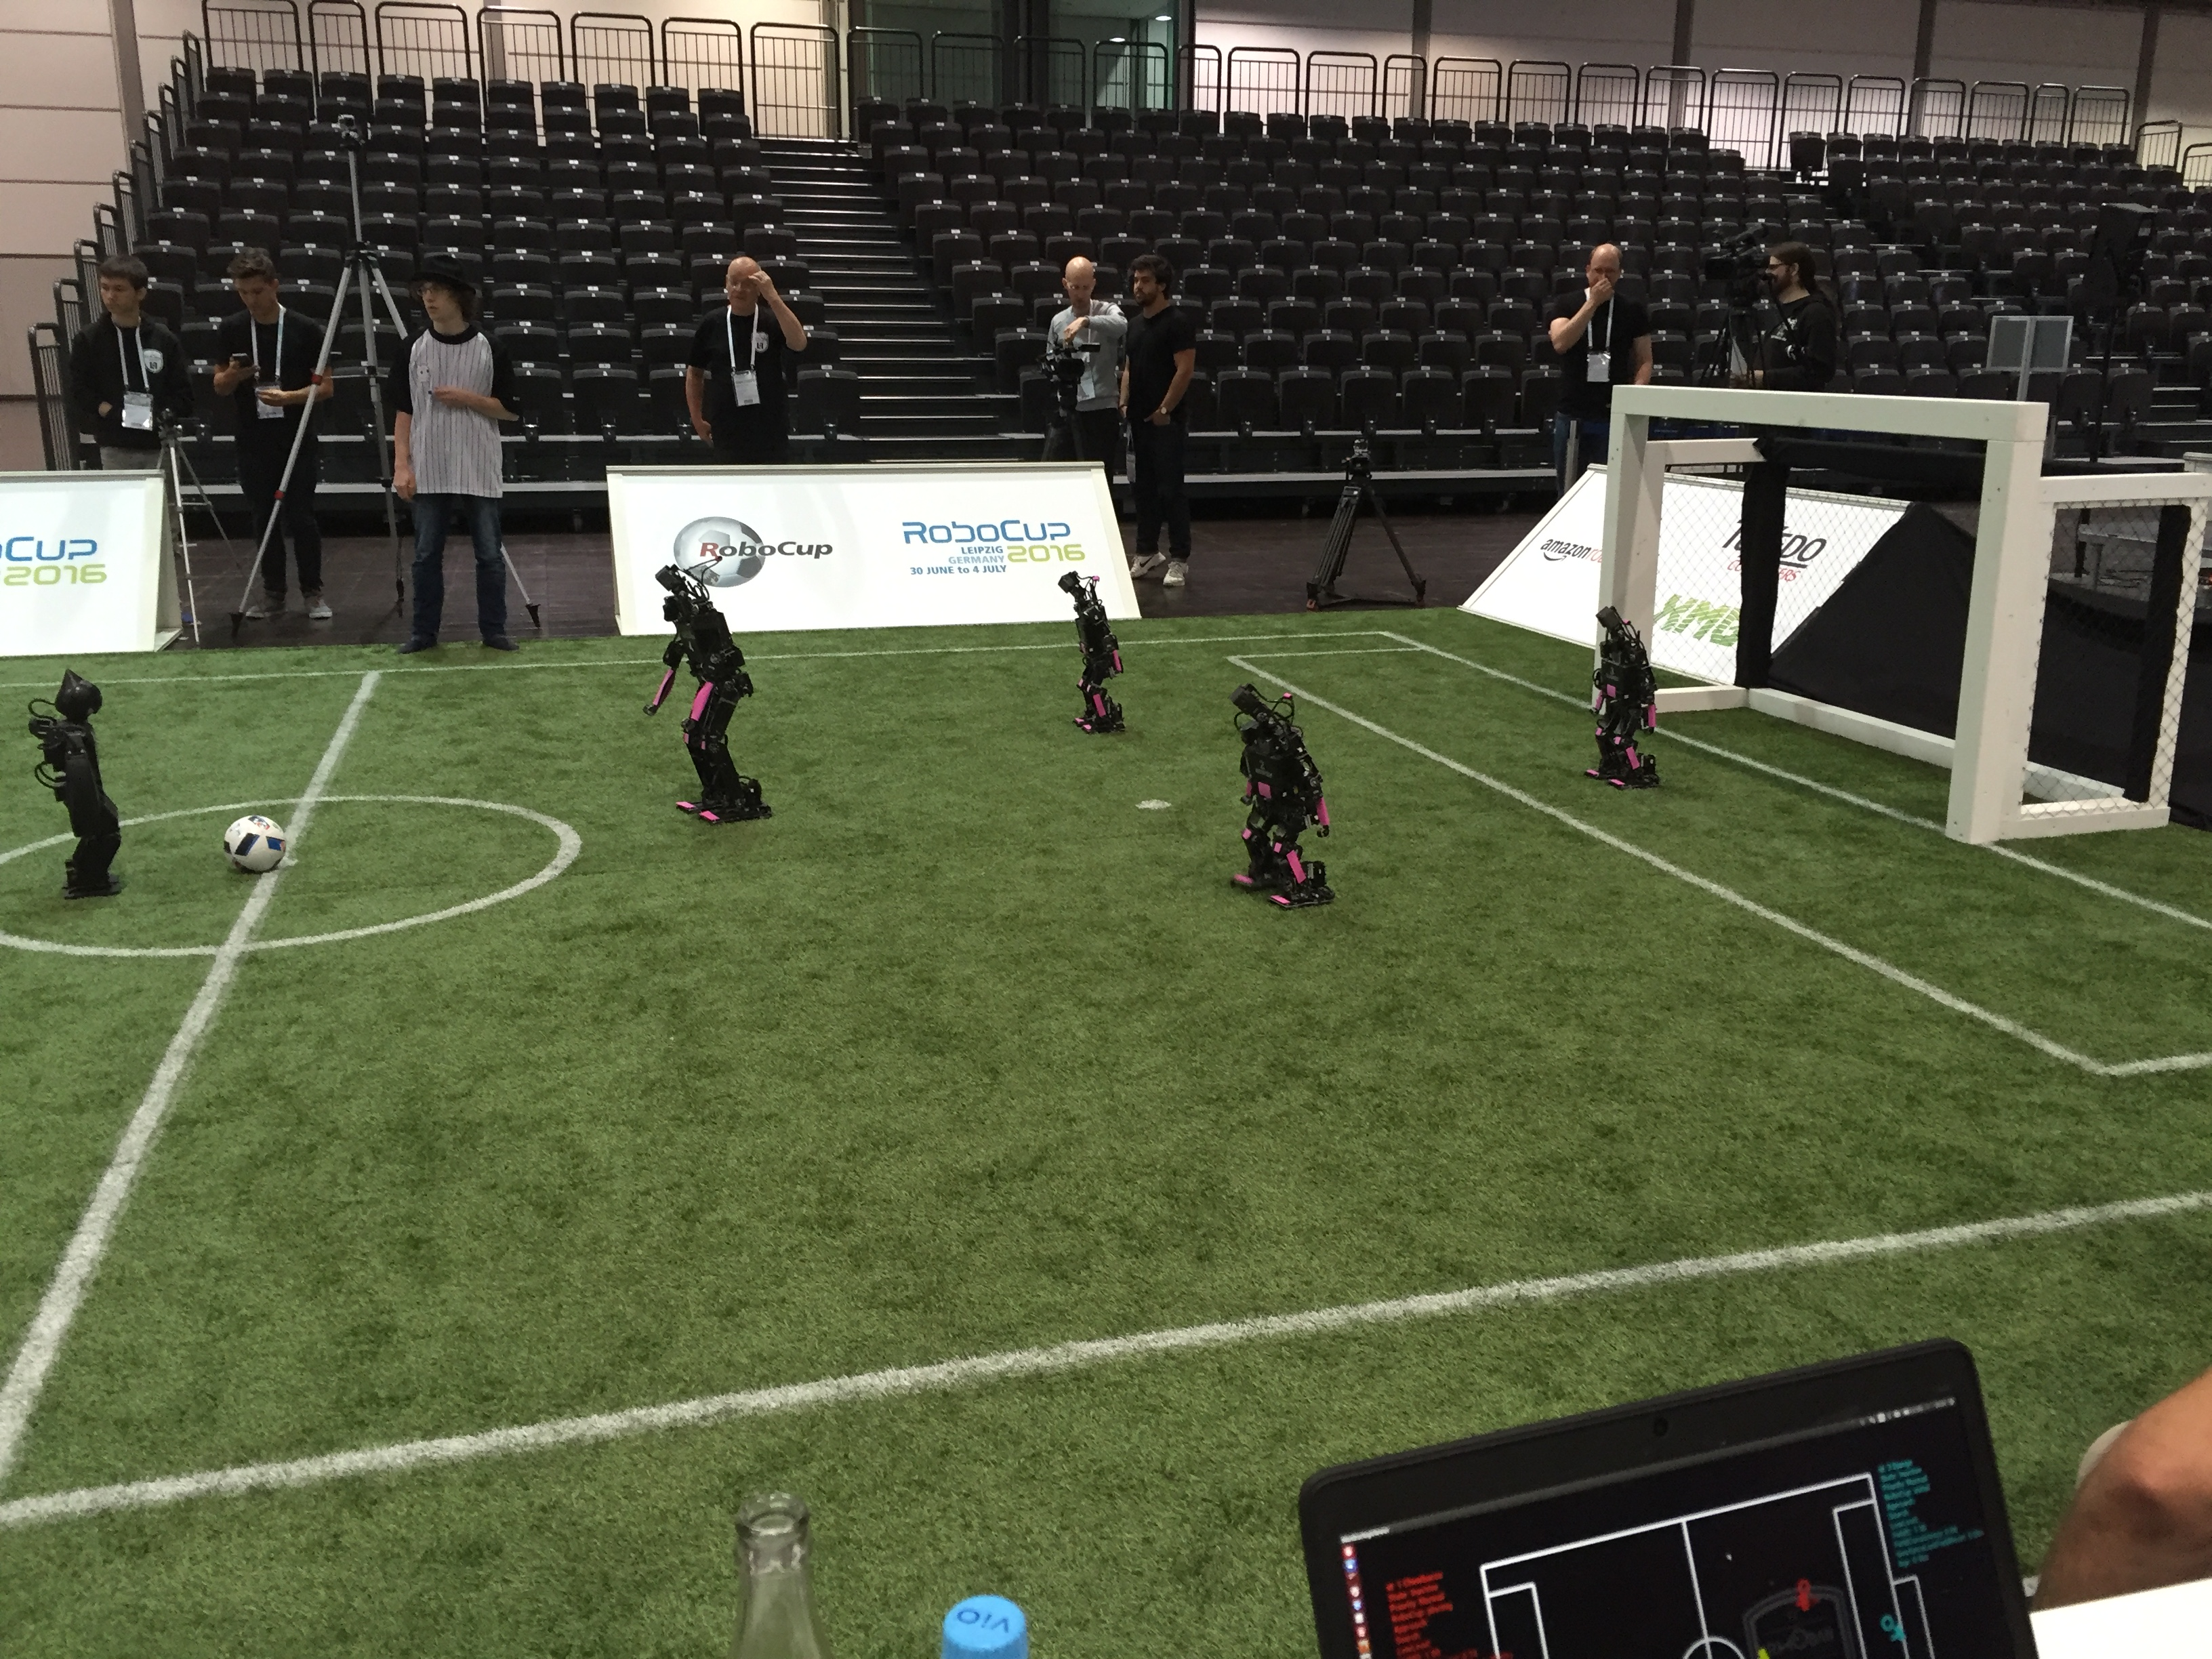
\includegraphics[width=1.0\linewidth]{../media/robocup_field.jpg}
    \end{subfigure}
    \begin{subfigure}{0.43\paperwidth}
        \centering
        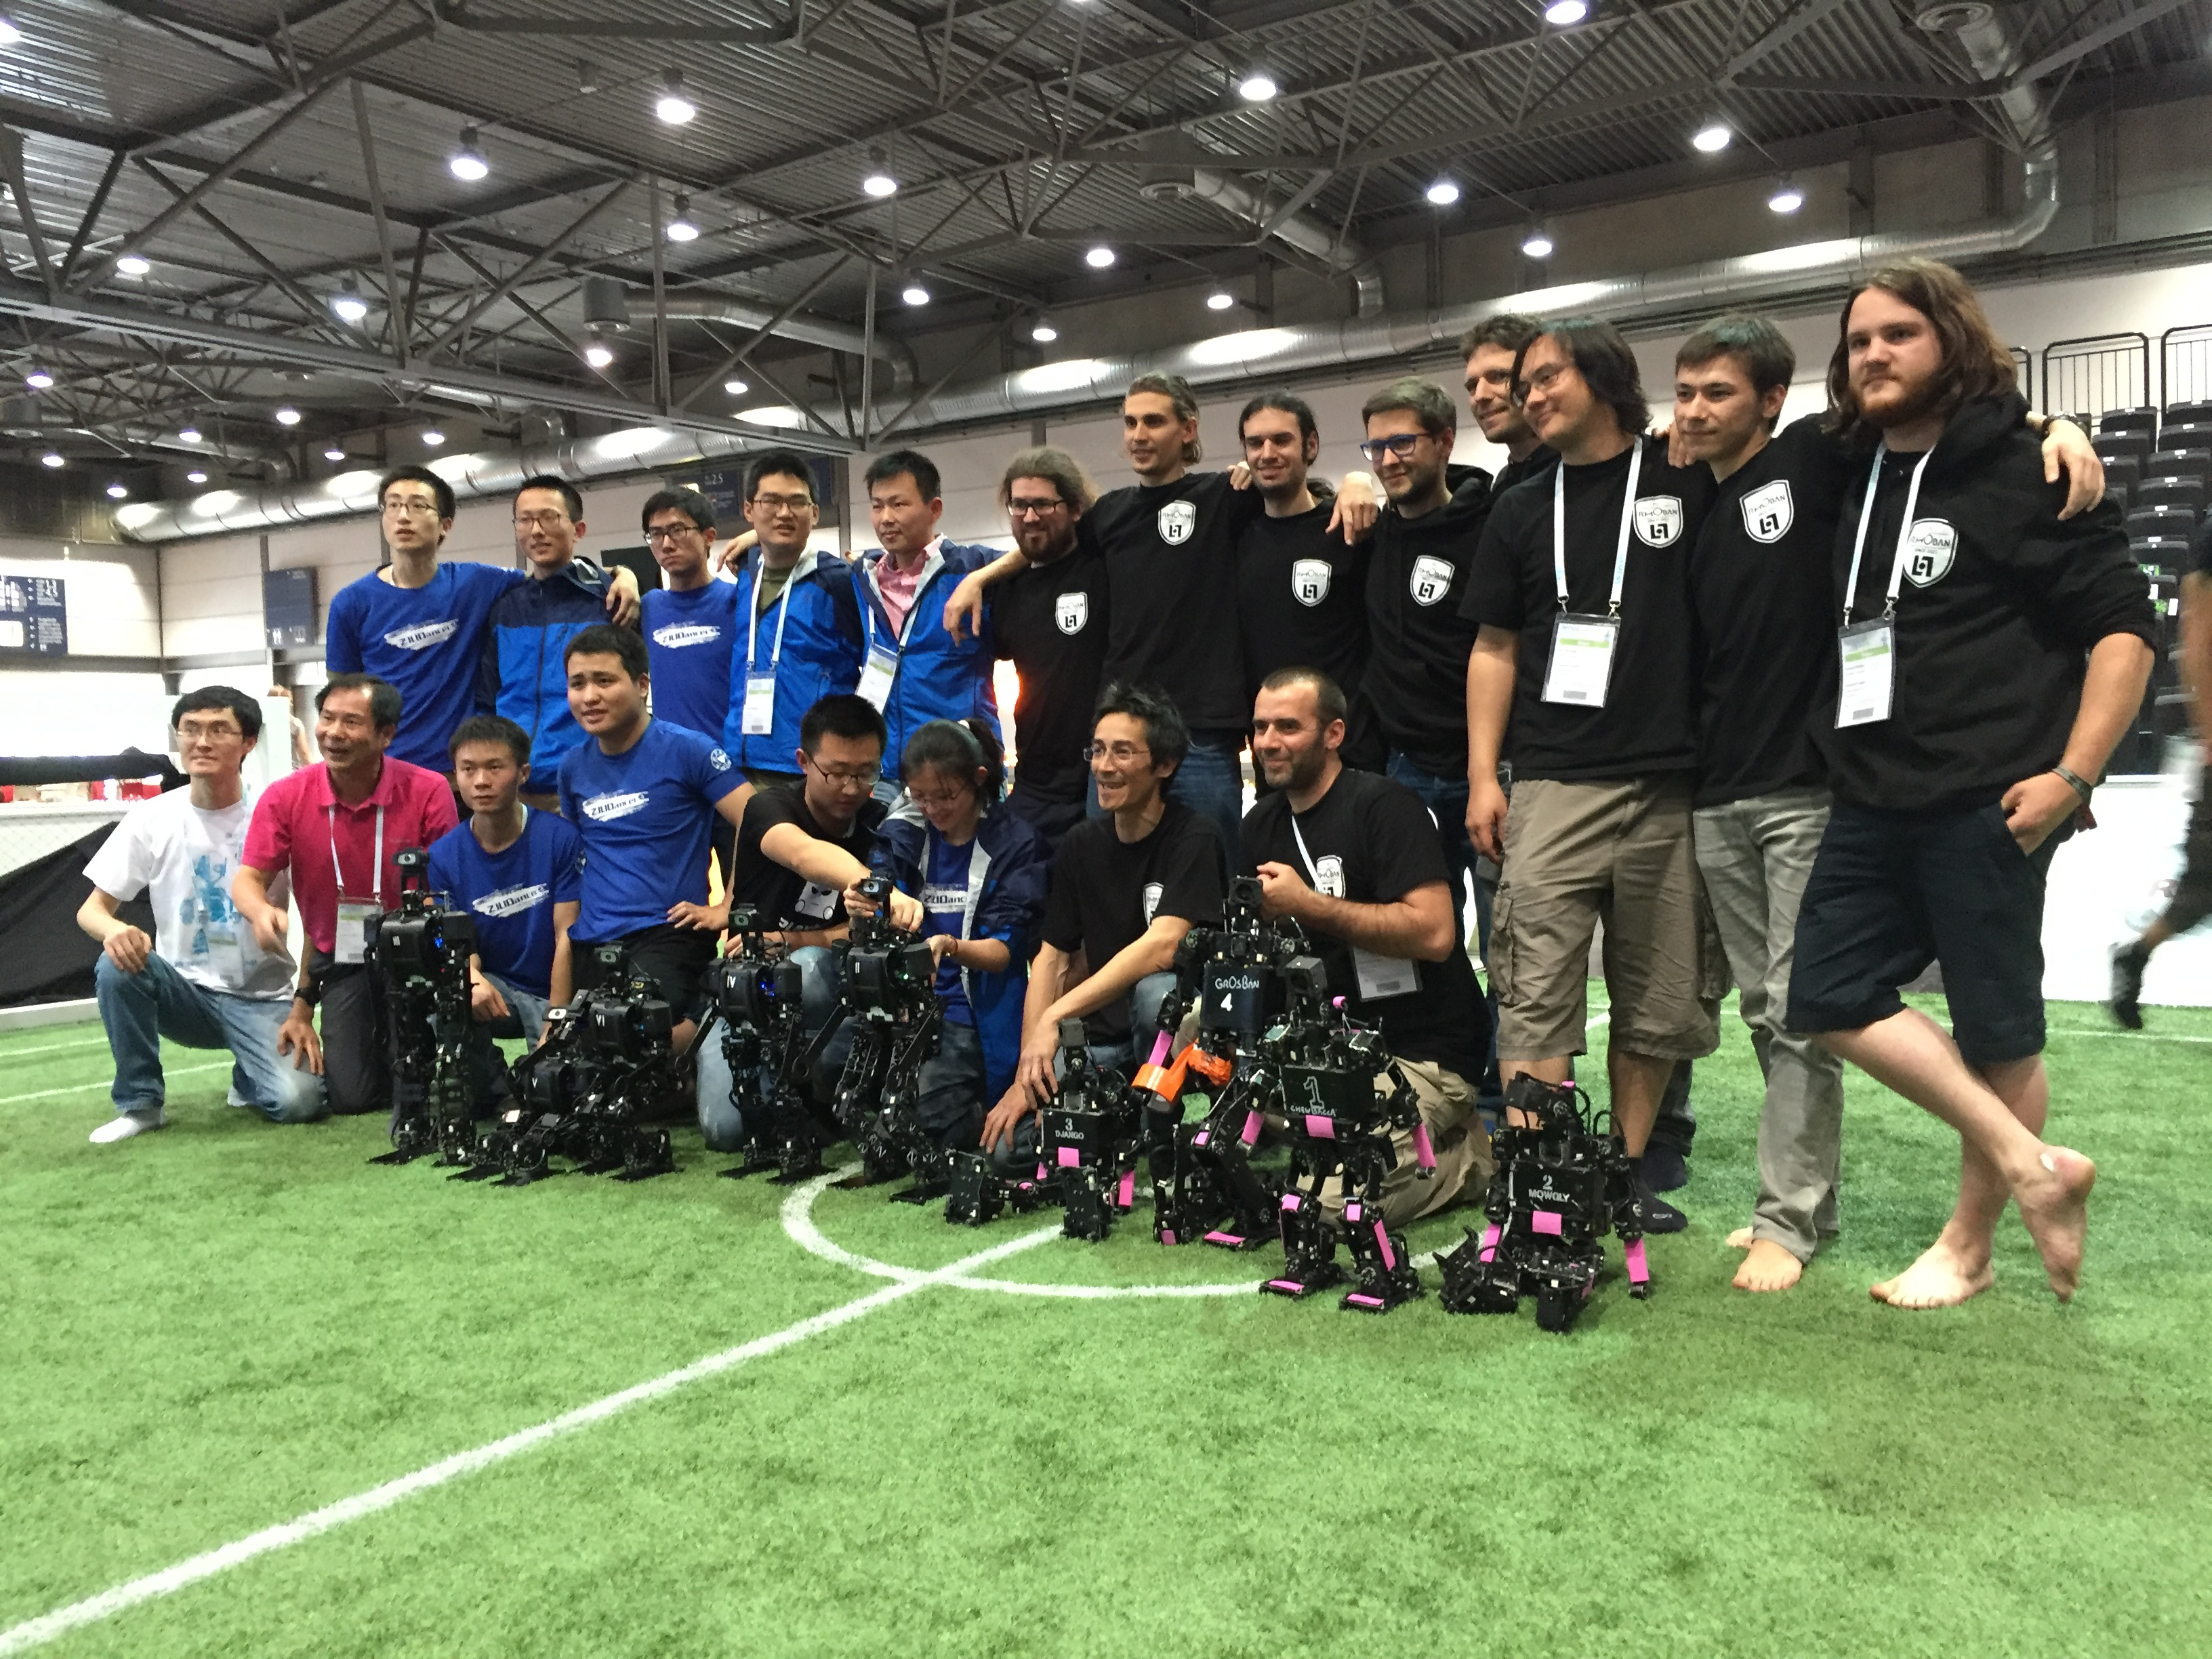
\includegraphics[width=1.0\linewidth]{../media/robocup_team.jpg}
    \end{subfigure}
    \caption{\label{fig:robocup} 
        Compétition RoboCup 2016 à Leipzig (Allemagne).
    }
\end{figure}

Par exemple, la ligue AIBO active de 1999 à 2008 a vu s'affronter
des équipes de petits robots quadrupèdes autonomes. 
De nombreuses techniques utilisées aujourd'hui ont été initialement
expérimentées sur ces robots.
Cette ligue constituée de robots \og standards \fg, a depuis été remplacée
par celle des petits robots humanoïdes NAO.

La compétition se joue également sur des robots à roues omnidirectionnels.
Sans les problèmes liés à la motricité des humanoïdes, 
ces ligues se concentrent sur des problématiques plus \og haut niveau \fg 
telles que la planification, le jeu en équipe et la perception.
La ligue \textit{Middle-Size} sur des grands robots à roues autonomes 
d'environ $80$~cm de haut, réalise déjà chaque année un match
contre une équipe humaine amateur.
Sur des robots à roues plus petits et très rapides, 
la ligue \textit{Small-Size} s'affranchit des problèmes de perception
par une localisation visuelle et externe.
Le contrôle de tous les robots est alors centralisé sur un ordinateur déporté.
On peut également mentionner l'existence de ligues en simulation.
La ligue 2D travaillant sur des aspects purement stratégiques et stochastiques
et la ligue 3D se rapprochant de la ligue standard NAO mais 
sans les contraintes du monde physique.

L'équipe Rhoban concourt quant à elle à la ligue \textit{Humanoid} créée 
à partir de 2002 et dont l'historique ainsi que les perspectives 
sont résumées par \cite{gerndt_humanoid_2015}.
Cette ligue se divise encore en trois catégories en fonction de la taille 
des robots y participant.
Les grands robots \og adultes \fg (\textit{Adult-Size}) de plus de $130$~cm, 
les robots de taille intermédiaire (\textit{Teen-Size}) entre $80$ et $140$~cm,
et enfin les robots de petites tailles (\textit{Kid-Size}) de moins de $90$~cm.
C'est dans cette dernière catégorie et regroupant le plus d'équipes que participe 
l'équipe Rhoban sous le nom du \textit{Rhoban Football Club}.
Contrairement à la ligue standard, les robots de cette ligue ne sont pas imposés
et sont le plus souvent conçus et construits par chacune des équipes participantes.
La contrainte majeure de cette ligue est qu'elle impose l'anthropomorphisme des robots.
En plus de contraintes géométriques sur la morphologie des robots, il est interdit
d'employer des capteurs n'ayant pas d'équivalent chez l'humain.
Typiquement, la mesure de distances par ultrasons, la perception du champ magnétique, 
l'utilisation de radars lasers (LIDAR) ou encore la vision du spectre infrarouge 
ne sont pas autorisés.

À noter que d'année en année, le règlement de la ligue évolue,
en convergeant progressivement vers le règlement officiel de la FIFA.
La complexité technique de la compétition augmente graduellement, 
sous la volonté d'atteindre aux alentours des 2050, le niveau 
requis par l'ambition originale (\cite{baltes_robocup_2014}).\\

L'intérêt de cette compétition internationale de football 
robotique autonome est loin de n'être que ludique.
La conception et la programmation d'un robot humanoïde footballeur font
intervenir de nombreuses problématiques de recherche très actuelles :
conception mécatronique, locomotion bipède, 
intelligence sensori-motrice, perception et localisation 
dans un environnement dynamique, stratégie de jeu en équipe, etc.

L'autre principal intérêt de cette compétition est 
d'offrir un contexte \og \textit{adversarial} \fg et très \textit{opérationnel}
pouvant être utilisé pour comparer différentes 
approches techniques (\cite{behnke_robot_2006}, \cite{anderson_robotics_2011}).
À l'origine, les premiers robots n'ont été déployés que dans des conditions
très contrôlées, comme des usines ou des laboratoires de recherches.
Un des enjeux majeurs de la robotique d'aujourd'hui est de réussir à 
faire opérer les robots dans des environnements de moins en moins contrôlés, 
avec pour objectif typiquement le domicile des particuliers, 
les zones urbaines ou les terrains extérieurs accidentés.
Un terrain de football est un bon exemple d'environnement 
semi contrôlé.

Enfin, il faut souligner la forte contrainte opérationnelle qu'impose le contexte
de la compétition à la fois sur les équipes, mais également sur les solutions
techniques mises en œuvres.
Il ne s'agit pas de développer une technique fonctionnant une seule fois, 
après de nombreux réglages dans un laboratoire.
Il faut pouvoir mette au point une technique qui fonctionnera à chaque fois, 
à l'heure dite, robuste aux conditions matérielles toujours un peu aléatoires, 
et capable d'être déployée en une journée à l'autre bout du monde.\\

Le développement de l'équipe Rhoban, sa montée collective en compétences
ont été fortement stimulés par cette compétition.
Après plusieurs années où de gros efforts d'ingénierie ont été consentis 
par tous (et le sont encore), l'introduction graduelle d'éléments de \og recherche \fg état de l'art
a permis une forte progression des résultats de l'équipe.
Le parcours du \textit{Rhoban Football Club} peut se résumer ainsi :
\begin{itemize}
    \item[2011,]Istanbul (Turquie).\\
        Toute première participation 
        sous le nom, \og \textit{Sigmaban Football Club} \fg.
    \item[2013,]Eindhoven (Pays-Bas).\\
        Deuxième participation sous 
        le nom d'équipe actuel, \textit{Rhoban Football Club}.
        Pour la première fois, l'équipe est en mesure
        de faire participer trois robots humanoïdes robustes
        sans problème matériel majeur.
        Le premier but de l'équipe est marqué par la tête 
        d'un des robots en tombant sur la balle.
    \item[2014,]Jo\~ao Pessoa (Brésil).\\
        Avec un mouvement de marche robuste, une meilleure perception
        et un comportement de jeu plus évolué,
        l'équipe fait un bond en avant en atteignant
        les quarts de finale.
    \item[2015,]Hefei (Chine).\\
        L'équipe parvient à bien s'adapter aux modifications des règles :
        remplacement de la surface de marche par de l'herbe artificielle
        et suppression des couleurs de la balle et des poteaux de but.
        En atteignant les demies finales, l'équipe prend la
        troisième place de la compétition.
    \item[2016,]Leipzig (Allemagne).\\
        L'équipe remporte la première place 
        de la ligue \textit{Humanoid Kid-Size}
        grâce à son système de vision flexible, l'amélioration de son
        module de localisation, la précision de son l'odométrie ainsi
        que l'ébauche d'un jeu d'équipe haut niveau.
    \item[2017,]Nagoya (Japon).\\
        Pour la seconde fois, l'équipe Rhoban atteint la première place
        et remporte de plus le prix du meilleur robot humanoïde.
\end{itemize}
J'ai eu la chance de pouvoir personnellement participer 
aux éditions de 2013 à 2016 (figure \ref{fig:robocup}). 
Je me suis également partiellement impliqué dans la préparation de l'édition 2017.

\section{Des robots imparfaits mais robustes}

L'équipe Rhoban conçoit et construit le petit robot humanoïde
Sigmaban. Malgré tout le soin apporté à sa réalisation, ce robot
est soumis à de nombreux défauts ou imperfections :
Avec l'usure et le temps, ses pièces mécaniques tendent 
à se déformer, du jeu apparait au niveau de ses articulations
et des problèmes électriques affectent le comportement des moteurs.
Il faut savoir de plus que le mouvement du robot est créé par 
des servomoteurs commerciaux.
Bien que très pratiques dans leur utilisation et leur disponibilité, 
ces moteurs soufrent de graves problèmes d'asservissement : 
il est ainsi très délicat de faire suivre précisément aux articulations
du robot une trajectoire définie à l'avance.
Pour résumer, le robot ne se comporte pas comme l'on souhaiterait qu'il
se comporte. Il est difficile de le contrôler.

Même si cette dualité est artificielle et exagérée,
on peut regrouper les robots humanoïdes dans deux grandes catégories :
les robots \og précis \fg et les robots imparfaits.
Le robot Sigmaban et plus généralement la grande majorité des robots participant à
la compétition RoboCup humanoïdes appartiennent à cette seconde catégorie.

Les robots humanoïdes sont des systèmes mécaniques complexes.
La philosophie à l'oeuvre lors de la conception de ces robots \og précis \fg,
est, le plus possible, de rapprocher le comportement réel du robot
de sa modélisation mathématique.
Ainsi, l'application des méthodes théoriques est rendue bien plus aisée.
Dans la grande majorité des cas, la motorisation de ces robots est
spécialement conçue et adaptée à son architecture mécanique.
Les systèmes de réductions harmoniques (bien plus complexes que des engrenages) 
utilisés ne comportent pas de jeu mécanique.
Enfin, la mécanique et l'électronique mis en oeuvre sont très précises
et de très bonne qualité.
En conséquence, l'ordre de grandeur du coût de ces robots avoisine 
au minimum les 100000 euros (parfois bien plus).
Par exemple, on peut mentionner les robots de grande taille ASIMO et HRP-2 
ainsi que HOAP-3 pour les robots de taille similaire à Sigmaban.

À l'inverse, le coût des petits robots humanoïdes \og imparfaits \fg 
concourant dans la ligue RoboCup \textit{Kid-Size} n'excède 
que rarement les 10000 euros.
Leur petite taille impose de fortes contraintes sur
les possibilités d'intégration mécanique.
Les réducteurs harmoniques et les servomoteurs spécifiquement conçus
ne sont souvent pas assez miniaturisés pour répondre aux fortes 
contraintes d'encombrement de ces robots.
Ainsi la grande majorité des équipes fait appel à des servomoteurs
commerciaux dont la production est industrialisée.

Imparfaits et moins précis, ces petits robots se distinguent 
cependant par leur grande robustesse.
À quelques rares exceptions notables, les grands robots mécaniquement
très précis sont également très fragiles.
Les réducteurs harmoniques supportent par exemple très mal 
les chocs. 
Il est typiquement exceptionnel d'observer ces robots se déplacer
sans être sécurisés par un palan les accompagnant.
Leur chute est accidentelle\footnote{La chute des robots humanoïdes étant 
néanmoins inéluctable dans un contexte opérationnel, différents travaux 
ont étudiés le contrôle et l'amortissement de telles chutes.} 
et ils ne sont en aucun cas prévus pour.

En comparaison, notre robot Sigmaban est bien plus résistant.
Les matchs de football robotique sont parfois mécaniquement très violents
pour nos robots. Les chutes et les collisions entre robots sont fréquentes.
C'est d'ailleurs précisément ces chocs qui tendent à altérer la 
structure mécanique.
Ce type \og d'accrochages brutaux \fg entre robots n'a pour le moment 
jamais été observé avec de grands robots autonomes.
Le principal avantage de leur grande robustesse, est de simplifier
et d'encourager les expérimentations sur le robot physique.
Par exemple sans être sécurisé, le robot peut être piloté
pendant de longues périodes de marche afin d'enregistrer son comportement.
De même, les mouvements (marche, tir, relevage) peuvent
être facilement et avec peu de risques mis au point directement 
sur le robot.

Néanmoins, pour pouvoir contrôler avec efficacité le robot,
il faut tout de même lutter contre ces imperfections.
L'idée de base de ces travaux de thèse est alors d'étudier la compensation 
des défauts de ces petits robots à l'aide de techniques d'apprentissage.
Ces techniques reposant justement sur l'acquisition de nombreuses données 
expérimentales afin de capturer puis corriger le comportement réel des robots. 

\section{Odométrie et mouvements de tir}

Outre une part importante d'ingénierie, les travaux
de thèse présentés ici se sont concentrés sur deux points 
directement en lien avec la compétition RoboCup.\\

Premièrement, la précision de l'odométrie du robot est améliorée.
L'odométrie est la capacité du robot à estimer son
propre déplacement au cours du temps. Deux odométries sont en réalité étudiées.
L'odométrie proprioceptive se base sur la lecture des capteurs du robot
alors que l'odométrie prédictive estime \og en simulation \fg le
déplacement futur du robot avant qu'il ne bouge réellement.
Pour la première, le problème consiste par exemple à marcher
les yeux fermés pendant quelques instants, puis à deviner 
où l'on se trouve, en sachant l'endroit d'où l'on est parti.
Pour la deuxième, il s'agit de prévoir de faire un certain nombre
de pas, puis de prédire avant de commencé à marcher où l'on va se retrouver.

Ces estimations sont toutes deux affectées par 
les nombreuses imperfections du robot.
Par exemple, les légères déformations mécaniques biaisent 
notre estimation proprioceptive du déplacement du robot.
D'autre part, les erreurs de suivi de trajectoire des pieds 
au cours de la marche induisent de grands décalages sur
la prédiction du déplacement du robot.

Lors des matchs de football robotique, l'odométrie proprioceptive
est très utile au robot à deux niveaux.
Tout d'abord, la mesure des déplacements du robot tient une grande
place dans le processus de localisation. En sachant d'où il part
sur le bord du terrain et en accumulant ses déplacements, le robot
est capable d'estimer sa position sur le terrain.
Savoir se repérer sur le terrain de football est en effet 
une capacité essentielle à la mise au point de stratégies 
de jeu plus évoluées.
D'autre part, l'odométrie proprioceptive est utile 
au contrôle de la direction de marche. 
Si l'odométrie du robot était parfaite, il ne lui suffirait
par exemple de ne voir la balle qu'une seule fois de loin pour
pouvoir, \og les yeux fermés \fg, se positionner en face de 
la balle et de la tirer.

Quant à l'odométrie prédictive, elle peut également être utilisée
pour améliorer la vitesse d'approche de la balle par le robot.
Le déplacement du robot est en effet soumis à de nombreux aléas.
Grâce à l'odométrie prédictive, le robot peut par exemple anticiper
ces perturbations et planifier un chemin précis
et rapide pour tirer la balle dans une direction donnée.\\

Deuxièmement, la question de la synthèse automatique 
de mouvements est explorée ; et plus précisément, 
le problème du mouvement de tir dans la balle.

Jusqu'ici, tous les mouvements du robot (relevage, marche et tir)
sont créés manuellement. Une fois la forme du mouvement globalement 
implémentée, les détails sont ajustés par expérimentation sur le robot réel.
Cependant, ce procédé nécessite beaucoup de temps humain et doit être 
continuellement répété pour chacun des mouvements et sur chacun des robots.
Le problème est en soi difficile. Pour qu'un mouvement soit performant, 
il doit souvent être rapide et donc très dynamique. Sur les robots
humanoïdes, le principale problème vient alors de la stabilité bipède.
Un bon mouvement ne doit pas faire tomber le robot.

Ce problème est un sujet largement étudié depuis longtemps
sur les grands robots \og précis \fg.
Puisque leur comportement est proche de ce que prévoit la théorie, 
de nombreuses méthodes mathématiques peuvent alors être appliquées.
Dans ces travaux, nous avons testé une des approches classiques
consistant à générer un mouvement au travers d'optimisations numériques.
Dans les cas simples et peu dynamique, cette technique fonctionne en effet.
Par contre sous l'effet des imperfections, dès que le mouvement désiré 
augmente en puissance, le comportement réel du robot s'éloigne 
alors de trop du mouvement théorique.
Le résultat est simple : alors qu'il aurait en théorie dû conserver son équilibre, 
le robot est déstabilisé et tombe.
L'idée est alors d'utiliser un simulateur physique afin de modéliser ses
défauts et d'apprendre le comportement réel du robot.
Les mouvements sont ensuite optimisés au sein de ce simulateur afin de tenir
compte des imperfections.
Cette idée est loin d'être nouvelle mais a peu été appliquée aux 
robots humanoïdes de petite taille au regard des très nombreux défauts.

Afin de prendre en compte la diversité des imperfections,
la réimplémentation d'un simulateur dynamique pour nos robots a été commencé.
Ces travaux sur la correction de la synthèse de mouvement ne sont toutefois
pas achevés. Ce manuscrit présente les détails théoriques nécessaire
à la mise en oeuvre d'une telle approche. Une grande partie des implémentations
logicielles sont aujourd'hui terminées, mais de nombreuses expérimentations restent 
à effectuer.

\section{Organisation du document}

Pour commencer, la section \ref{sec:robot} introduit la plateforme
robotique humanoïde Sigmaban, sur laquelle repose les travaux de cette thèse.
Conçue et construite par l'équipe Rhoban, progressant chaque année, 
un petit historique met en lumière les grandes étapes de cette évolution.
Le matériel constituant ce robot est ensuite décrit. 
Puis l'ensemble des imperfections motivant les travaux présentés ici 
sont enfin détaillés et caractérisés.

Ensuite, les concepts nécessaires à la modélisation géométrique du robot
sont exposés à la section \ref{sec:model_geometric}.
Les modèles géométriques direct et inverse sont définis ainsi que les conventions
utilisées. De plus, l'estimation de l'état du robot à partir de ses différents capteurs 
et le processus d'intégration de l'odométrie sont abordés.

La section \ref{sec:walk} présente enfin le fonctionnement du mouvement de marche
\textit{IKWalk} implémenté au cours de cette thèse, puis utilisé sur tous les robots 
de l'équipe Rhoban jusqu'en 2016. Toutes les expériences sur l'odométrie
présentées ici font appel et sont donc fortement liées à ce mouvement de marche.\\

Le chapitre suivant présente de manière non exhaustive la littérature
de l'odométrie et de la planification de pas à la section \ref{sec:biblio_odometry}, 
des techniques de marche humanoïde à la section \ref{sec:biblio_walk}, et enfin les
efforts de synthèse de mouvements, principalement par optimisation ou concernant
le mouvement de tir de la balle sur les robots humanoïdes, section \ref{sec:biblio_motion}.
Une des spécificités de la compétition RoboCup est qu'elle
fait appel à de nombreux domaines, tous très riches avec pour l'ambition 
de rassembler, d'appliquer et de comparer, à l'occasion d'un jeu de football robotique, 
le meilleur de l'état de l'art de chacun.\\

Le quatrième chapitre rentre dans les détails des principales contributions de
cette thèse sur la correction de l'odométrie.
La section \ref{sec:odometry_intro} commence par définir les deux types d'odométries, 
proprioceptive et prédictive analysées dans la suite.
La section \ref{sec:odometry_pressure} démontre le grand intérêt de l'utilisation
des capteurs de pression sous les pieds du robot, pour la qualité de l'estimation
de l'odométrie proprioceptive.

Enfin, les sections \ref{sec:odometry_lwpr} et \ref{sec:odometry_cmaes} présentent 
chacune les travaux ayant fait l'objet de deux publications.
La première apprend la correction des odométries par une technique de régression
non paramétrique et en se basant sur un dispositif de capteurs externes mesurant
la position absolue sur robot sur le sol.
Grâce à ce matériel, une comparaison approfondie des effets sur l'odométrie
des surfaces de marche (moquette et herbe artificielle) est menée.

Malheureusement, ce dispositif expérimental est impossible à mettre en oeuvre
en pratique dans le contexte de la compétition RoboCup.
La deuxième contribution expérimente alors une autre approche de correction
appliquée avec succès lors de l'édition 2016 de la RoboCup.
Les paramètres d'un modèle de correction linéaire sont identifiés par optimisation.
De plus, ces travaux en collaboration avec Ludovic Hofer abordent le problème
de la planification d'une politique de contrôle de la marche.
Ceci permettant d'accélérer le temps de positionnement et de tir du robot 
devant la balle.\\

Le cinquième chapitre aborde quant à lui le problème
de la synthèse de mouvement en présence d'imperfections.
À noter que même si les travaux concernant l'odométrie et ceux
abordant la synthèse de mouvement ont représenté dans cette thèse 
un temps d'élaboration équivalent, ces derniers mobilisent des 
concepts bien plus complexes.
Ces travaux sont encore en cours de développement 
et seuls quelques premiers résultats sont aujourd'hui connus.
Dans la présentation qui en est faite, l'accent est mis ici 
sur la description des multiples points techniques clefs.
Les premiers résultats ne sont que très brièvement mentionnés.

La section \ref{sec:model_dynamics} présente ainsi les différents 
concepts et algorithmes nécessaires à la modélisation 
du comportement dynamique du robot.
Plus précisément, ces concepts sont appliqués d'une part, à
l'évaluation de la stabilité d'un mouvement par dynamique inverse.
D'autre part, à l'implémentation d'un simulateur physique (dynamique directe)
du robot gérant en particulier les contacts avec le sol.

Enfin, la section \ref{sec:motion_generation} expose la méthode 
suivie pour la génération de mouvements par optimisation.
Le choix de la représentation des mouvements et les critères 
d'évaluation de leurs performances y sont notamment évoqués.\\

Pour terminer, la section \ref{sec:publications_and_works} liste et résume
succinctement les publications issues de cette thèse.
Les autres travaux entrepris au sein et pour l'équipe Rhoban mais 
n'ayant pas pu être décrits ici sont également rapidement évoqués. 

Enfin, la section \ref{sec:perspectives} ouvre aux nombreuses 
perspectives restant à explorer :
l'amélioration toujours possible de la plateforme robotique, 
le perfectionnement de l'estimation de l'odométrie
et surtout la synthèse de mouvement au travers d'un simulateur
fondé (\og \textit{grounded} \fg) sur la réalité.\\

